\section{Experiments}
\subsection{Experimental Setup}
In our experiments, we used the  Bayesian Network shown in Figure~\ref{fig:alarm_fig} as a base model for structure learning and probability estimation. The network, as shown in Figure~\ref{fig:alarm_fig}, models relationships between various variables and provides a realistic test case for Bayesian network learning.

We performed simulations by generating datasets of varying sizes (ranging from 5 to 10,000 samples) based on the dependencies in the network. These datasets were then used to learn the Bayesian Network structures and the probability distributions associated with them, followed by an evaluation of the learned networks.\footnote{We provide the experiments and necessary codes to reproduce our results in the github repository: \url{https://github.com/pratik2358/bayes_net_learning}}
\begin{figure}[htp!]
\begin{center}
\begin{minipage}{0.3\textwidth}
\[
P(E) :
\begin{array}{|c|c|}
\hline
E & P(E) \\
\hline
t & 0.01 \\
f & 0.99 \\
\hline
\end{array}
\]
\end{minipage}%
\begin{minipage}{0.3\textwidth}
\[
P(B) :
\begin{array}{|c|c|}
\hline
B & P(B) \\
\hline
t & 0.2 \\
f & 0.8 \\
\hline
\end{array}
\]
\end{minipage}%
\begin{minipage}{0.35\textwidth}
\[
P(R \mid E) :
\begin{array}{|c|c|c|}
\hline
E & P(R = t) & P(R = f) \\
\hline
t & 0.6 & 0.4 \\
f & 0.05 & 0.95 \\
\hline
\end{array}
\]
\end{minipage}%

% \vspace{1em}

\begin{minipage}{0.3\textwidth}
\[
P(A \mid E, B) :
\begin{array}{|c|c|c|c|}
\hline
E & B & P(A = t) & P(A = f) \\
\hline
t & t & 0.99 & 0.01 \\
t & f & 0.9 & 0.1 \\
f & t & 0.97 & 0.03 \\
f & f & 0.14 & 0.86 \\
\hline
\end{array}
\]
\end{minipage}
\hfill
\begin{minipage}{0.35\textwidth}
\[
P(C \mid A) :
\begin{array}{|c|c|c|}
\hline
A & P(C = t) & P(C = f) \\
\hline
t & 0.7 & 0.3 \\
f & 0.01 & 0.99 \\
\hline
\end{array}
\]
\end{minipage}
\end{center}
\centering
    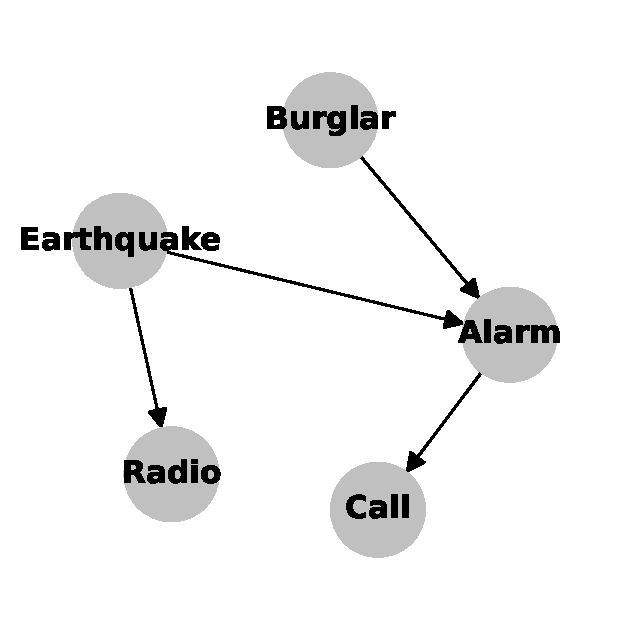
\includegraphics[width=0.5\linewidth]{plots/alarm.pdf}
    \caption{An example of a Bayesian Network to learn}
\label{fig:alarm_fig}
\end{figure}

\subsection{Results}
\begin{figure}[htp!]
     \centering
     \begin{subfigure}{0.7\textwidth}
         \centering
    
\includegraphics[width=\textwidth]{plots/legends.pdf}
     \end{subfigure}
     \begin{subfigure}{0.32\textwidth}
         \centering
         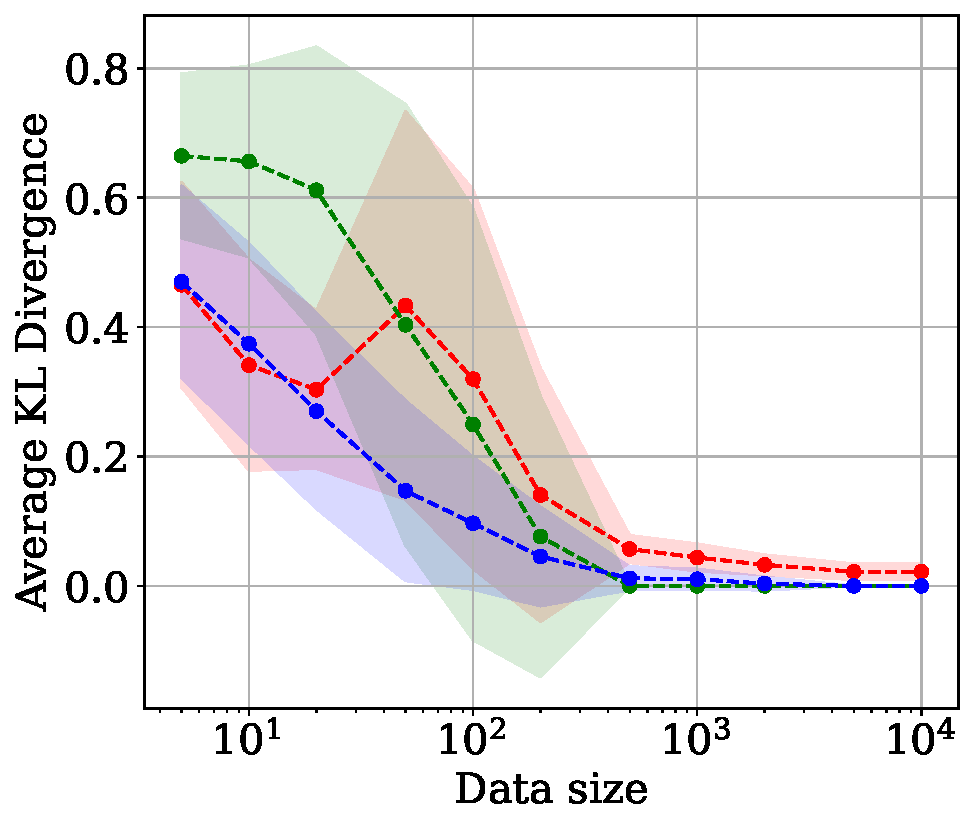
\includegraphics[width=\textwidth]{plots/kl_divergence.pdf}
         \caption{KL divergence between the probability distributions learned by the model and that observed in the data.}
         \label{fig:kl_div_dist}
     \end{subfigure}
     \hfill
     \begin{subfigure}{0.32\textwidth}
         \centering
         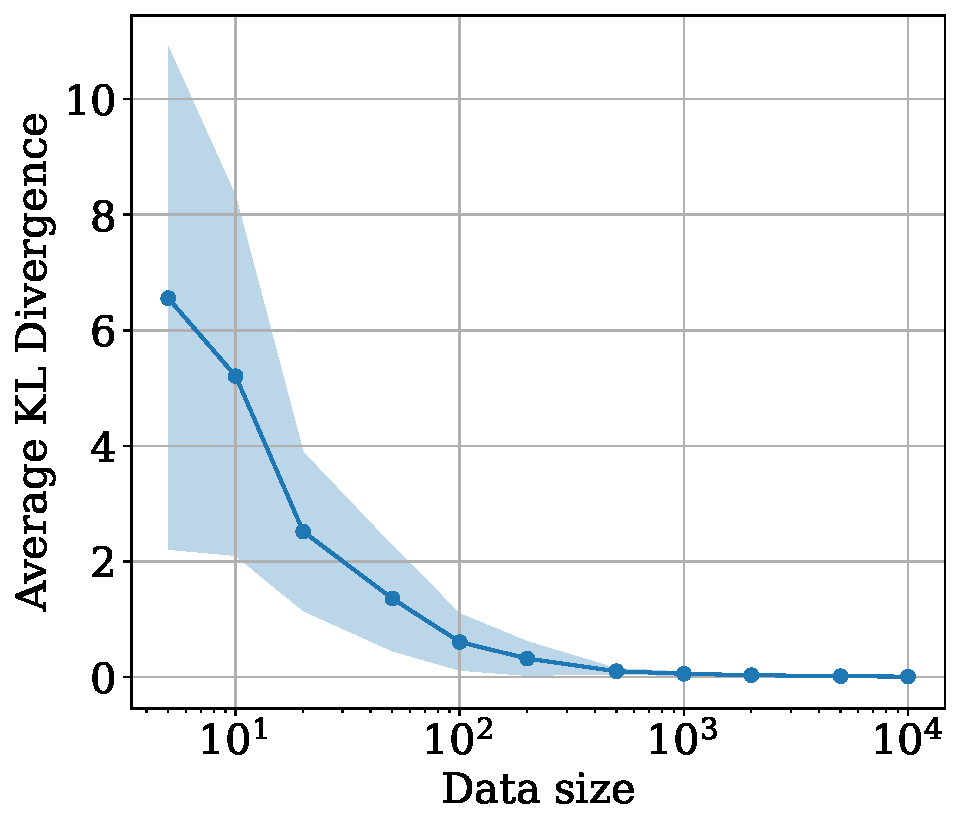
\includegraphics[width=\textwidth]{plots/joint_dist_div.pdf}
         \caption{KL divergence between the joint distributions observed from the samples from the model and that observed in the data.}
         \label{fig:kl_div_joint}
     \end{subfigure}
     \hfill
     \begin{subfigure}{0.32\textwidth}
         \centering
         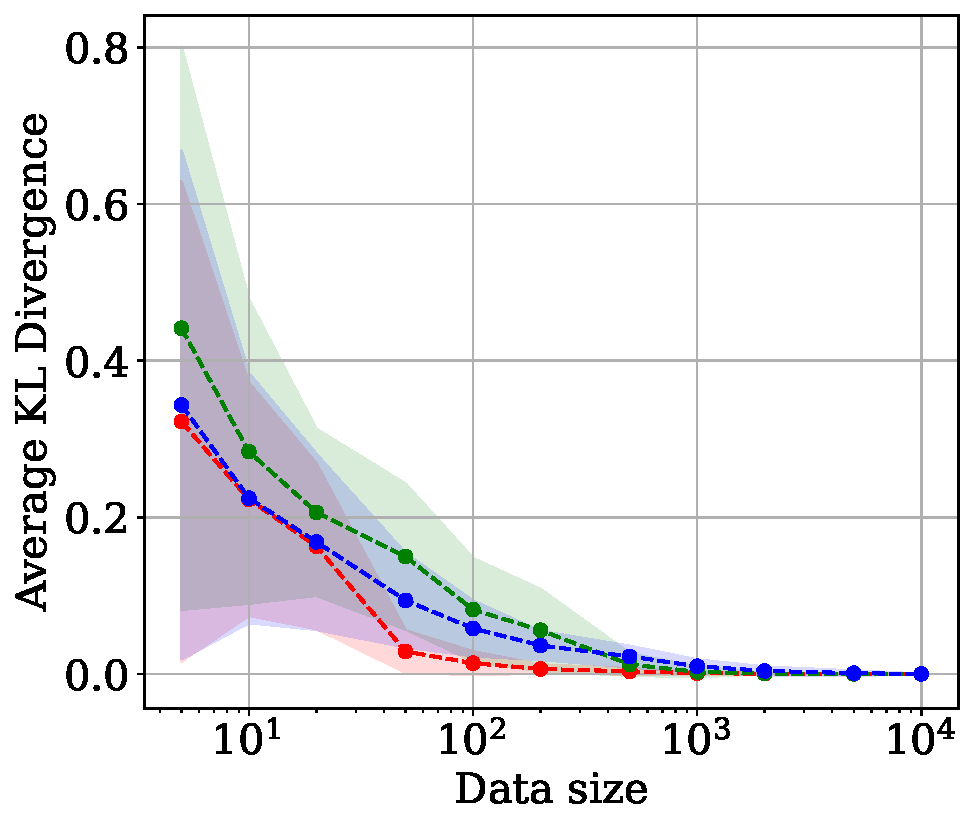
\includegraphics[width=\textwidth]{plots/conditionals_kl_divergence.pdf}
         \caption{KL divergence between the conditional distributions observed from the samples from the model and that observed in the data.}
         \label{fig:kl_div_conditionals}
     \end{subfigure}
        \caption{Comparison among Exact algorithm (unbounded number of parents and 2 maximum parents) and Chow-Liu approximation algorithm for learning Bayesian networks from discrete data.}
        \label{fig:str_learning_comp}
\end{figure}

\begin{figure}[htp!]
\begin{subfigure}{0.7\textwidth}
         \centering
    
\includegraphics[width=\textwidth]{plots/legends.pdf}
     \end{subfigure}
    \centering
    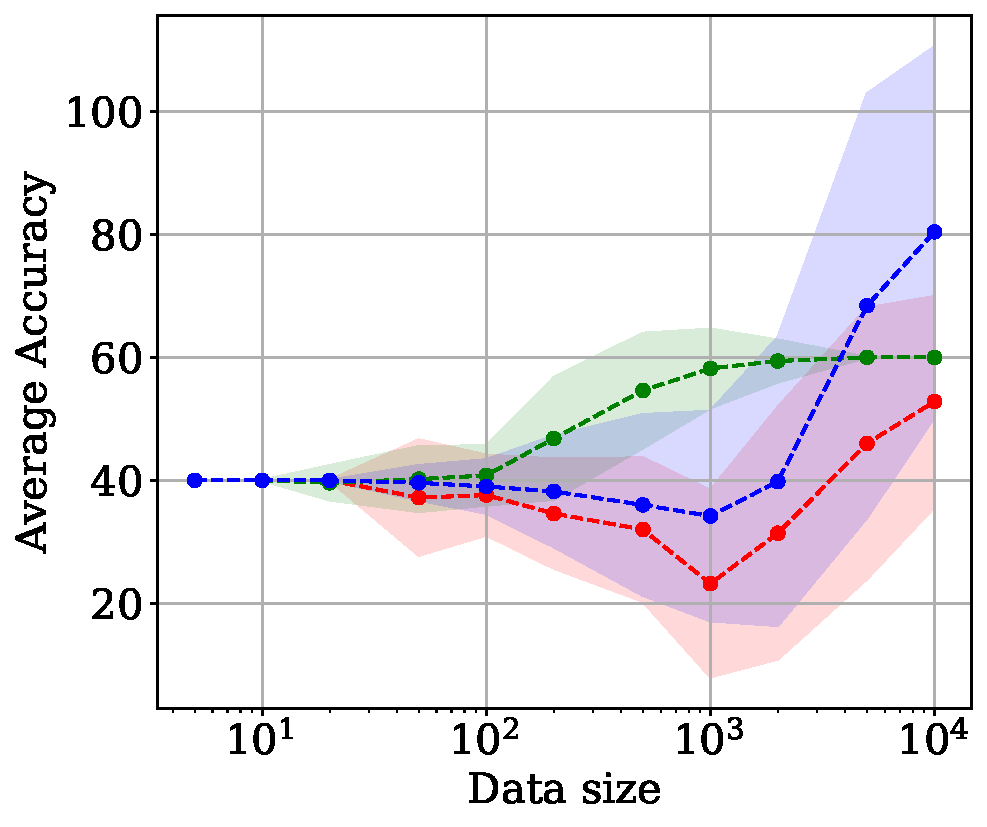
\includegraphics[width=0.5\linewidth]{plots/accuracy.pdf}
    \caption{Comparison of structural accuracy using Exact algorithm (unbounded number of parents and 2 maximum parents) and Chow-Liu approximation learning}
    \label{fig:str_acc}
\end{figure}

\begin{figure}[htp!]
    \centering
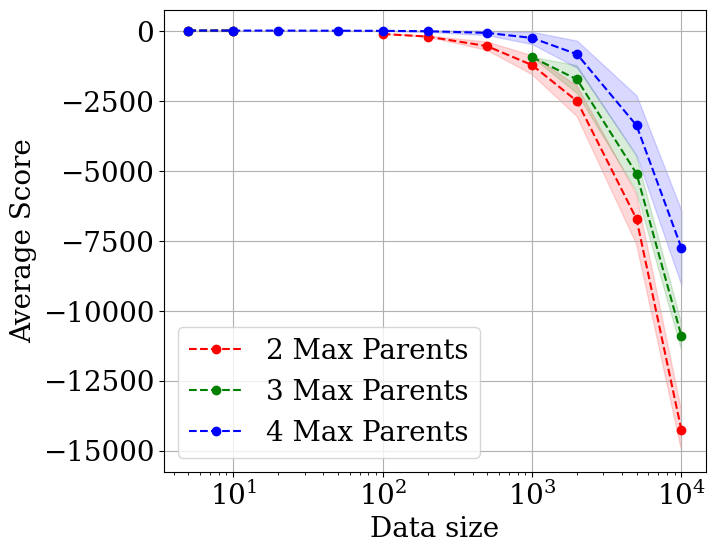
\includegraphics[width=0.5\linewidth]{plots/scores.png}
    \caption{Comparison of negative BIC scores using Exact algorithm for different number of maximum parents}
    \label{fig:bic}
\end{figure}